\section{Reconstructing distortion coefficients}
\subsection{The problem}
\subsection{The index grid}
Let $I \subset \mathbb{N}\times\mathbb{N}$ be a finite set. The elements of $I$ are tuples $(i_0,i_1)$.
Then we define the {\em index grid} with respect to $I$ as:
\begin{equation}
G_I = \left\{j \in \Rpow{3} | j = (i_0,i_1,0) \mathrm{\ where\ } (i_0,i_1) \in I\right\}
\end{equation}
$G_I$ describes a normalized, aligned grid in three-dimensional space as shown in fig.~\ref{fig:IndexGrid}.
We will call the elements of $G_I$ {\em grid points} and represent them by the symbol $\ji$ with $i\in I$.
Without going into details we demand that $G_I$ be sufficiently reasonable, i.e. not degenerate
and with lots of grid points, so that we can use it in order to determine lens distortion.
For numerical reasons, $(0,0)$ should be an element of $I$.
\begin{figure}[h]
\label{fig:IndexGrid}
\centering
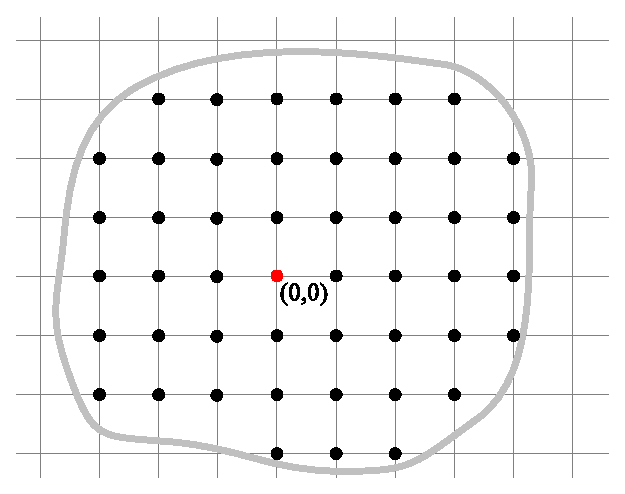
\includegraphics[width=5cm]{index_grid.eps}
\caption{Index grid ($xy$-plane) for a subset of $\mathbb{N}\times\mathbb{N}$}
\end{figure}
\subsection{Perspective transformation}
We consider the geometry of a standard camera with focal length $f$. This camera is located
in the origin of three-space and looking towards $-z$. The $x$- and $y$-axis of the image produced by this camera
coincide with the $x$- and $y$-axis in three-space projected into the image plane.
A point $(x,y,z)\in\Rpow{3}$ is projected into the image plane as follows:
\begin{align}
\label{PerspectiveProjection}
P_f^\mathrm{3d} &: \Rpow{3} \rightarrow \Rpow{3} \nonumber\\
    &:  \left(x,y,z\right) \mapsto \left(\frac {-fx}{z},\frac {-fy}{z},-f\right)
\end{align}
The result is a point in the image plane in length units (like $f$).





\subsection{The homogenious transformation}
Let us assume, we observe this grid through a standard camera (located at the origin, looking towards $-z$).
In order to model the real situation of a grid shot we have to scale, rotate and translate the grid and project it.
We use a scaling factor $S > 0$, a matrix $R$ and a vector $T$ for transforming as mentioned before.
Then we get the following. Now, according to (\ref{PerspectiveProjection}) each grid point $\ji$ is mapped into the image plane like
\begin{equation}
\ji \mapsto H_{S,R,T}(\ji) = \frac {-f(SR\ji + T)}{(SR\ji + T)_2}
\end{equation}

On the other hand, we have user input, namely the original tracking points of a grid shot within \tde.
Let us denote these points by $\piorigunit$. These points are positioned in the distorted image.
The method of finding the distortion coefficients is to try out various sets of distortion
coefficients $\{q\}$ and unwarp the points $\piorigunit$. In other words, we calculate
points $\piiterunit$ by unwarping $\piorigunit$ using the coefficients $\qset = \{q\}$:
\begin{equation}
\piiterunit(\qset,\lcounit) = \gq^{-1}(\piorigunit - \lcounit) + \lcounit
\end{equation}
Now we can construct a target function for an optimization procedure.
Again, $I\subset\mathbb{N}\times\mathbb{N}$ denotes the index set of our index grid.
\begin{equation}
F(\qset,\lcounit,S,R,T) = \sum_{i\in I}\left[\psi(\piiterunit(\qset,\lcounit)) - H_{S,R,T}(\ji)\right]^2
\end{equation}

Other form
\begin{equation}
F = \sum_{i\in I}\left[(c\cdot\ji+1)\piitercm - (a\ji+b)\right]^2 \wi
\end{equation}
This form of the target function has several advantages.
It is a quadratic form in $a$, $b$ and $c$, so that we can (at first sight)
easily minimize it with respect to $a,b,c$, and this enables us to implement
a derivative-based optimization procedure (e.g. using \Newton\ iteration)
